\documentclass{article}

\usepackage{graphicx}
\usepackage{fancyhdr}
\usepackage[sorting=none]{biblatex}
\usepackage[margin=1in]{geometry}
\usepackage{listings}
\usepackage[hidelinks]{hyperref}
\usepackage{xcolor}
\usepackage{xepersian}
\usepackage{ltablex}
\usepackage{booktabs, makecell, longtable}



\addbibresource{bibliography.bib}
\settextfont[Scale=1.2]{IRNazli.ttf}
\setlatintextfont[Scale=1]{times.ttf}
\renewcommand{\baselinestretch}{1.5}
\pagestyle{fancy}
\fancyhf{}
\renewcommand{\headrulewidth}{1pt}
\renewcommand{\footrulewidth}{1pt}
\setcounter{tocdepth}{1}
\begin{document}

\def\by{نگارش}
\def\superv{مدرس}
\def\faculty{دانشکده مهندسی کامپیوتر}
\def\course{رایانش عصبی}
\def\docTitle{پروژه ششم }
\def\supervisor{دکتر رضا صفابخش}
\def\fname{سیدمهدی }
\def\lname{میرفندرسکی}
\def\stuNum{401131065}
\def\docDate{دی 1401}

\rhead{\docTitle}
\lhead{درس \course}
\rfoot{\fname \lname}
\lfoot{\stuNum}
\cfoot{\\ \thepage}



\begin{titlepage}
\begin{center}
%
\includegraphics[width=0.4\textwidth]{fa-logo.png}\\
\centerline{{
\includegraphics[height=3.8cm]{fa-logo}}}        
\LARGE
%\textbf{دانشگاه صنعتی اصفهان}\\
%\textbf{دانشکده مهندسی کامپیوتر}\\
\bf{\fontsize{16pt}{16pt}\selectfont دانشگاه صنعتی امیرکبیر}\par
\fontsize{14pt}{15pt}\selectfont(پلی‌تکنیک تهران)\par
\fontsize{16pt}{17pt}\selectfont \faculty \par
        
\par
        

\vfill
{\huge\settextfont{B_Titr.ttf}{\docTitle  درس  \course}}
\vfill
 
\settextfont[Scale=1.2]{BNazanin.ttf}
{\huge\by}\\
\fontsize{18pt}{19pt}\selectfont\bfseries{\fname \lname} \\
\settextfont[Scale=1.2]{BNazanin.ttf}
{\huge\superv}\\
{\fontsize{18pt}{19pt}\selectfont\bfseries\par\supervisor}\\
\fontsize{16pt}{17pt}\selectfont\docDate\\
 
 
        
\LARGE
%\textbf{نام و نام خانوادگی: مجید فرهادی}\\
%\textbf{شماره دانشجویی: 9700000}\\
%\textbf{نیم‌سال تحصیلی: پاییز 1400}\\
%\textbf{مدرّس: دکتر محمّدرضا حیدرپور}\\
%\textbf{دستیاران آموزشی: مجید فرهادی - دانیال مهرآیین - محمّد نعیمی}\\
\end{center}
\end{titlepage}


\tableofcontents

\newpage

\section{سوال اول - تشریحی}

ساختار سلول \lr{LSTM} و \lr{GRU} به صورت زیر است:

\begin{figure}[!h]
    \centering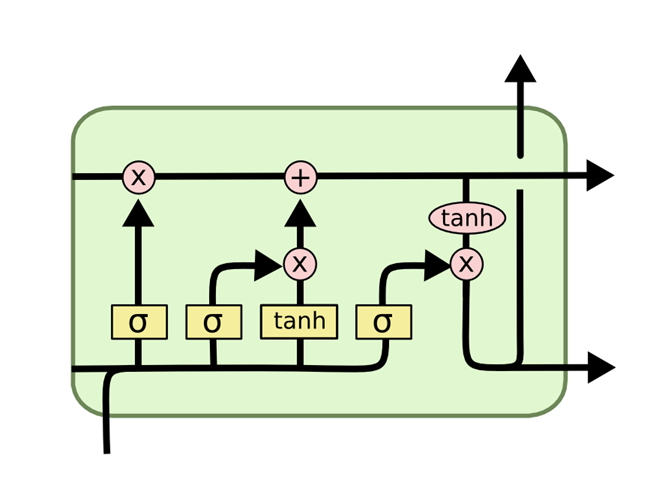
\includegraphics[scale=.55]{./i-1}
    \caption{معماری \lr{LSTM}}\label{fig.01}
\end{figure}
% \cleardoublepage
% همچنین ساختار سلول \lr{GRU} به صورت زیر است:
\begin{figure}[!h]
    \centering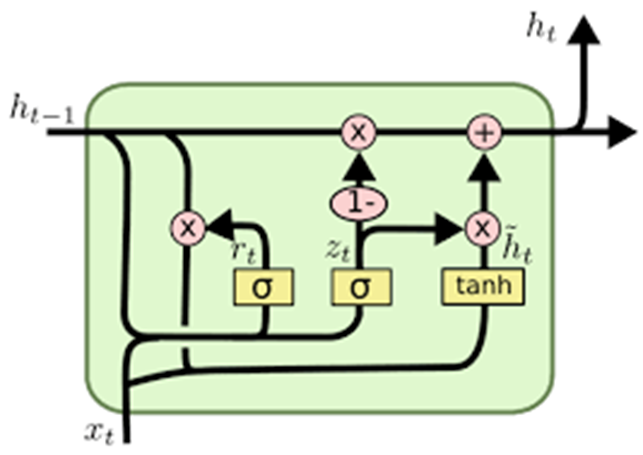
\includegraphics[scale=.55]{./i-2}
    \caption{معماری \lr{GRU}}\label{fig.01}
\end{figure}

\cleardoublepage

شباهت هر دو نوع شبکه در این است که هر دو با ارائه ساختاری بر  \lr{RNN} وضعیتی از زما‌ن‌های قدیم را حفظ کنند (یک واحد حافظه). نوشتن و خواندن این حافظه توسط شبکه یاد گرفته شود. اما جزییات پیاده‌سازی آن‌ها با هم متفاوت خواهد بود.  همانطور که در اشکال ارائه شده مشاهده می‌‌شود، سلول \lr{LSTM} دارای سه گیت است (\lr{Input}، \lr{Output} و \lr{Forget}). گیت \lr{Forget}  تعیین‌کننده تغییر یا عدم تغییر وضعیت سلول خواهد بود. گیت  \lr{Input} جریان ورودی را مشخص می‌کند و نهایتا گیت \lr{output} جریان خروجی بر اساس وضعیت فعلی را کنترل خواهد کرد. اما اساسا معماری و ساختار \lr{GRU} یک معماری ساده‌تر با بهره‌گیری از \lr{LSTM} است. دراین معماری دو گیت \lr{reset}  و \lr{update} وجود دارد. گیت \lr{update} اهمیت اطلاعات جدید را مشخص می‌کند و در وضعیت سلول جایگزین می‌شود و گیت  \lr{reset}  تعیین می‌کند اهمیت اطلاعات قبلی چقد است و آیا باید حفظ شود؟

با توجه به مطالب ذکر شده به نظر می‌رسد که \lr{GRU} هزینه محاسباتی کمتری داشته باشد. همچنین قابلیت تغییرپذیری آن بیشتر خواهد بود. اما طبیعتا قدرت \lr{LSTM} بیشتر خواهد بود. از طرفی \lr{LSTM} احتمال بیش برازشش بیشتر خواهد بود.

پشته‌کردن \lr{LSTM}: این کار با توجه به اینکه \lr{LSTM} ها بر روی داده‌های توالی کار می‌کنند، به این معنی است که با افزودن لایه‌ها سطوح انتزاعی مشاهدات ورودی را در طول زمان اضافه می‌کند. در واقع، مشاهدات را در طول زمان تکه تکه می‌کند یا مشکل را در مقیاسه‌های زمانی مختلف نشان می‌دهد. به بیان دیگر گفته‌شده، این رویکرد به طور بالقوه به حالت پنهان در هر سطح اجازه می‌دهد تا در مقیاس زمانی متفاوتی عمل کند.
پشته‌کردن \lr{GRU}: مطالب بیان شده برای \lr{LSTM} برای این قسمت نیز صادق خواهد بود. 

اما باید توجه شود که پشته‌کردن \lr{LSTM} مدل را بیش از اندازه پیچیده خواهد کرد. این بدان خاطر خواهد بود که سلول \lr{LSTM} به تنهایی پیچیده است و با اینکار آموزش شبکه سخت‌تر خواهد شد زیرا درحال حاضر شبکه‌ای خواهیم داشت که هر لایه آن به اندازه کافی پیچیده خواهد بود. اما در معماری \lr{GRU} چون معماری ساده‌تری دارد آموزش مقداری راحت‌تر خواهد بود.



% -------------------------------------------------------------------

\section{سوال دوم - تشریحی}
گرادیان در این سلول شامل بردار فعال‌سازی‌های دروازه فراموشی است که به شبکه اجازه می‌دهد تا مقادیر گرادیان‌ها را در هر مرحله زمانی با استفاده از به‌روزرسانی‌های پارامتر مناسب دروازه فراموشی کنترل کند. وجود فعال‌سازی‌های دروازه فراموشی به سلول این امکان را می‌دهد تا در هر مرحله زمانی تصمیم بگیرد که اطلاعات خاصی فراموش نشود و پارامترهای مدل را متناسب با آن به‌روزرسانی کند. پس می‌توان برای اینکه گرادیان ناپدید نشود، یک به روزرسانی برای پارامتر دروازه فراموشی در مرحله زمانی  بعدی پیدا کنیم که مشتق جزئی خطا نسبت به وزن در زمان بعدی صفر نشود. پس در نهایت وجود پارامتر دروازه فراموشی این امکان را در هر زمانی فراهم می‌آورد. و در نهایت مشکل از بین رفتن گرادیان حل می‌شود.
% -------------------------------------------------------------------

\section{سوال سوم - تشریحی}
بله، شبکه های حافظه کوتاه مدت بلند را می‌توان به صورت موازی و توزیع شده آموزش داد. آموزش موازی شامل استفاده از چندین منبع پردازشی برای آموزش مدل به طور همزمان است که می‌تواند روند آموزش را سرعت بخشد. برای آموزش موازی کارهای زیر می‌تواند صورت گیرد:

\begin{itemize}
    \item موازی‌سازی داده‌ها (تقسیم داده‌ها به دسته‌های مختلف و پردازش هر یک در ماشین متفاوت)
    \item موازی‌سازی مدل (تقسیم مدل به لایه‌های مختلف و پردازش هریک در ماشینی مجزا)
    \item ترکیب روش‌های فوق
\end{itemize}

با این کار می‌توان مدل‌های بزرگتری و یا مدلی با داده‌های بیشتری آموزش داد. همچنین سرعت آموزش نیز افزایش می‌یابد. البته برای این کار نیاز به ماژول‌های جانبی خواهد بود (برای مدیریت).

% -------------------------------------------------------------------



\section{سوال اول}
پیش‌پردازش‌های اعمالی بر متن انواع گوناگونی دارد. در این بخش به همان موارد ذکرشده در صورت پروژه بسنده شد. همانطور که در ادامه مشاهده می‌شود، ابتدا علائم نگارشی را حذف کرده، سپس تمام حروف را کوچک و فواصل اضافی را حذف می‌کنیم. سپس کار را با حذف تگ‌های \lr{html} و لینک‌ها ادامه می‌دهیم. در نهایت نیز از متن باقی کلمات پرتکرار را حذف و متن را تبدیل به لیستی از کلمات می‌کنیم.


\begin{figure}[!h]
    \centering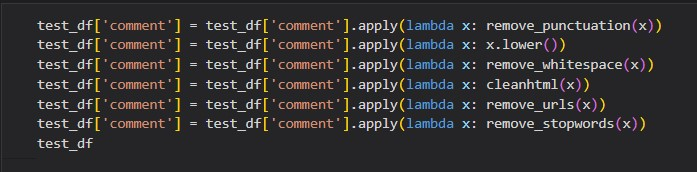
\includegraphics[scale=.75]{./p1-1}
    \caption{پیش‌پردازش متن}\label{fig.11}
\end{figure}

% -------------------------------------------------------------------

\section{سوال دوم}
\lr{one hot encoding} برای تعبیه کلمات توصیه نمی‌شود، زیرا اساسا طول هر بردار آن به اندازه طول کل دیکشنری خواهد بود. یعنی ما ورودی‌هایی خواهیم داشت که به شدت \lr{sparse} خواهند بود. این اتفاق هزینه محاسباتی مدل را بسیار افزایش خواهد داد.

\lr{Word2Vec} یک شبکه عصبی کم عمق و دو لایه است که برای بازسازی زمینه‌های زبانی کلمات آموزش داده شده است. این روش با استفاده از مجموعه بزرگی از کلمات به عنوان ورودی، یک فضای برداری را تولید می‌کند. به بیان دیگر هر کلمه منحصر به فرد به یک بردار متناظر در فضا نگاشت می‌شود. اما این بردارهای کلمه در فضای برداری به گونه‌ای قرار می‌گیرند کلمات مشابه نزدیک به هم باشند. 
این روش به صورت، مدل \lr{Continuous Bag-of-Words (CBOW)} و مدل \lr{Skip-Gram} عرضه می‌شود. به صورت دقیقتر \lr{Word2Vec} یک شبکه عصبی ساده با یک لایه پنهان است و مانند همه شبکه‌های عصبی دارای وزن است و در طول آموزش هدفش تنظیم آن وزن‌ها برای کاهش یک تابع هزینه است. با این حال، \lr{Word2Vec} قرار نیست برای کاری که در آن آموزش داده شده است استفاده شود، در عوض، فقط وزن‌های پنهان آن درنظر گرفته می‌شود.

در رابطه با پارامترهایی که باید تعیین شوند: اندازه پنجره هرچه بیشتر باشد به معنا بیشتر توجه می‌کند اما از طرفی زمان آموزش بیشتر خواهد شد. ما در اینجا اندازه پنجره را 5 درنظر گرفتیم (میانه). همچنین چون مجموعه داده ما بسیار بزرگ نیست، لازم نیست از مقادیر بزرگ برای اندازه بردار ویژگی استفاده کنیم. مقدار 100 برا آن در نظر گرفته شد. 

% -------------------------------------------------------------------

\section{سوال سوم}

این قسمت نکته خاصی ندارد، جز اینکه از روش دوم استفاده شد و حد آستانه 90 درصد داده‌ها تعیین شد. بدین ترتیب جملات با حدود طول 242 درنظر گرفته شدند.


% -------------------------------------------------------------------

\section{سوال چهارم}


برای سعی و خطا این قسکت شبکه‌های زیر بررسی شد و نتایج آن در ادامه قابل مشاهده است. در این قسمت در ابتدا سعی شد اکثر حالت‌های ممکن بررسی شوند (معماری دوسویه، پشته‌ای و ...) اما حجم داده‌ها بسیار زیاد بود به همین دلیل به اجرای 4 نوع شبکه بسنده شد (هر نوع سلول 2 شبکه). برای آموزش شبکه‌ها مجبور به ذخیره مدل، داده‌های آموزشی و داده‌های آزمون شدیم. همچنین با توجه به نوع مسئله ترجیح داده شد که از معماری دو طرفه استفاده شود. همچنین برای هر سلول یک شبکه با یک لایه و یک شبکه با دو لایه ایجاد شد. برای لایه‌های پنهان نیز از 4 لایه استفاده کردیم (با لایه خروجی). این شبکه‌ها با 10 ای‌پاک آموزش داده شدند.

معماری چهار شبکه ذکر شده به همراه نمودارها و همچنین ماتریس درهم ریختگی آن در ادامه مشاهده می‌شود.


\begin{figure}[!h]
    \centering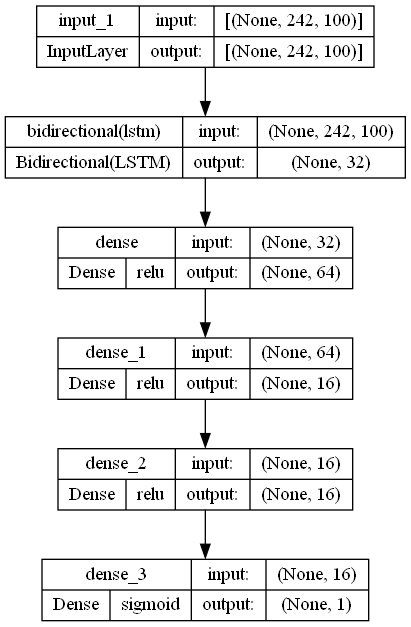
\includegraphics[scale=.45]{./LSTM-[16]}
    \caption{\lr{LSTM-[16]-[64, 16, 16]}}\label{fig.41}
\end{figure}


\begin{figure}[!h]
    \centering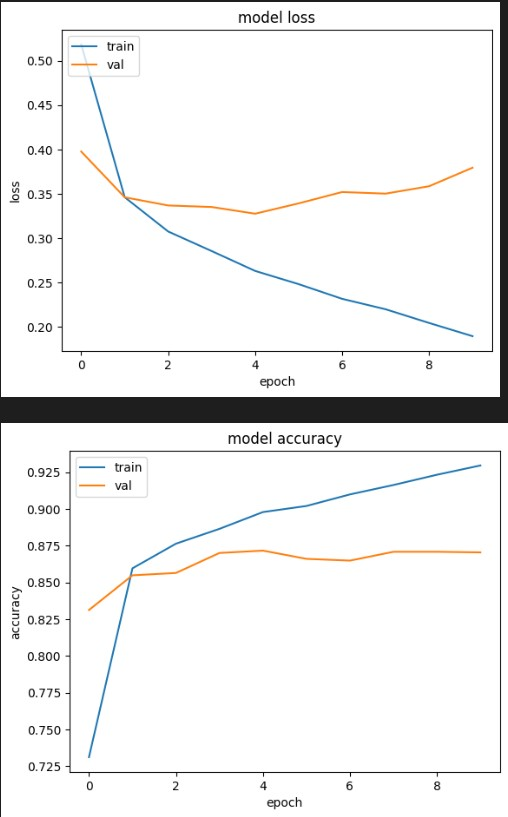
\includegraphics[scale=.65]{./LSTM-[16]-[64, 16, 16]}
    \caption{\lr{LSTM-[16]-[64, 16, 16]}}\label{fig.42}
\end{figure}


\begin{figure}[!h]
    \centering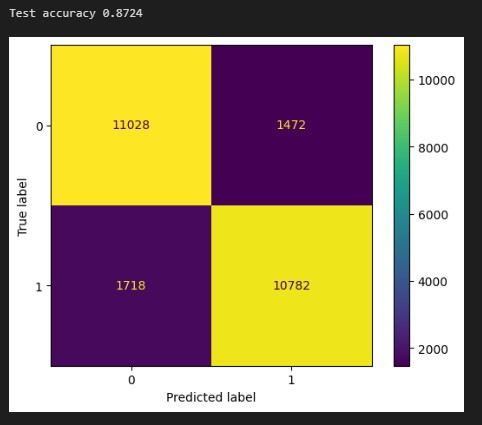
\includegraphics[scale=.70]{./test-LSTM-[16]}
    \caption{\lr{LSTM-[16]-[64, 16, 16]}}\label{fig.43}
\end{figure}





\begin{figure}[!h]
    \centering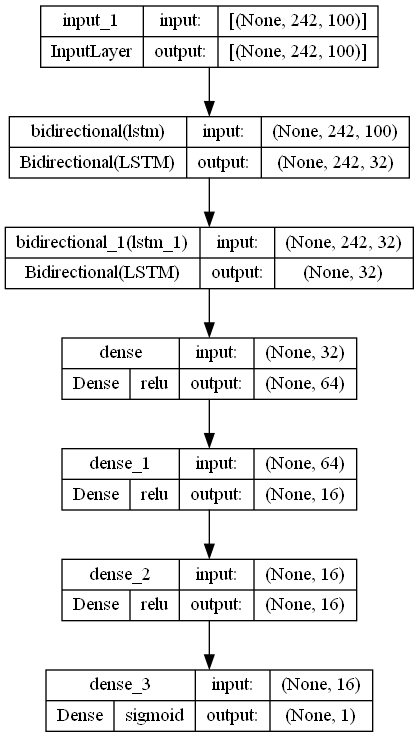
\includegraphics[scale=.45]{./LSTM-[16, 16]}
    \caption{\lr{LSTM-[16, 16]-[64, 16, 16]}}\label{fig.44}
\end{figure}


\begin{figure}[!h]
    \centering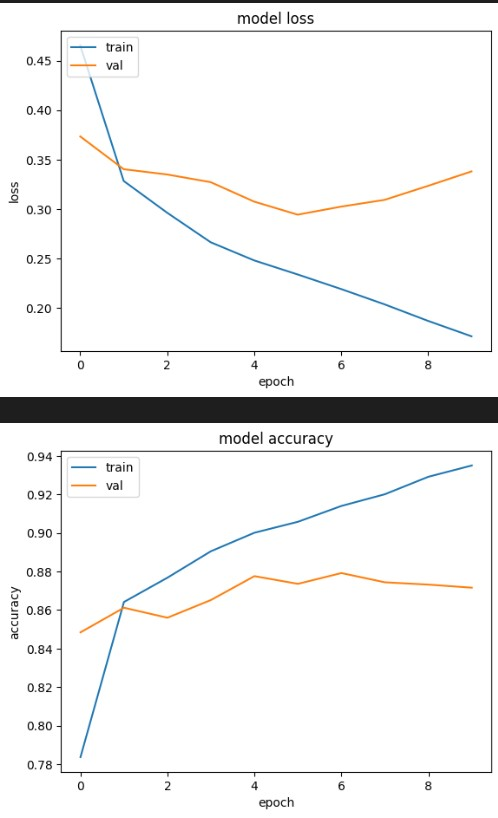
\includegraphics[scale=.65]{./LSTM-[16, 16]-[64, 16, 16]}
    \caption{\lr{LSTM-[16, 16]-[64, 16, 16]}}\label{fig.45}
\end{figure}


\begin{figure}[!h]
    \centering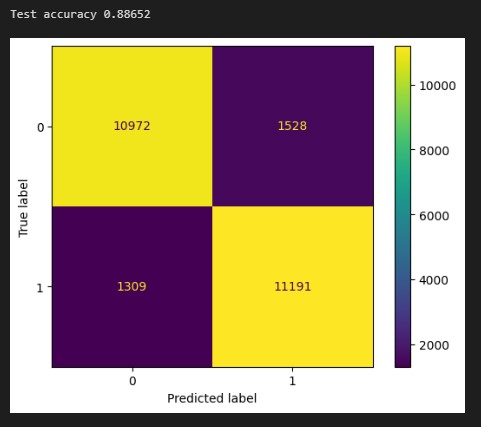
\includegraphics[scale=.70]{./test-LSTM-[16, 16]}
    \caption{\lr{LSTM-[16, 16]-[64, 16, 16]}}\label{fig.46}
\end{figure}

% \lr{LSTM-[16]-[64, 16, 16]}

% \lr{LSTM-[16, 16]-[64, 16, 16]}




% \lr{GRU-[16]-[64, 16, 16]}

% \lr{GRU-[16, 16]-[64, 16, 16]}



\begin{figure}[!h]
    \centering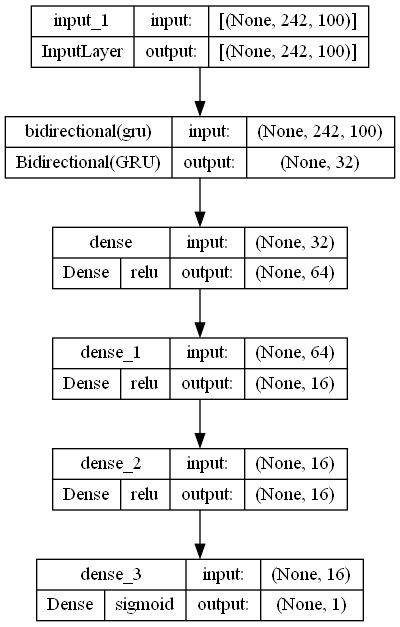
\includegraphics[scale=.45]{./GRU-[16]}
    \caption{\lr{GRU-[16]-[64, 16, 16]}}\label{fig.47}
\end{figure}


\begin{figure}[!h]
    \centering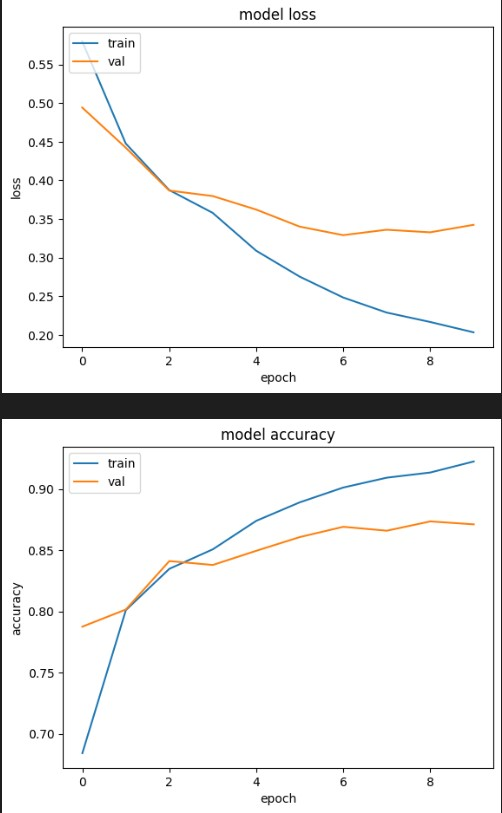
\includegraphics[scale=.65]{./GRU-[16]-[64, 16, 16]}
    \caption{\lr{GRU-[16]-[64, 16, 16]}}\label{fig.48}
\end{figure}


\begin{figure}[!h]
    \centering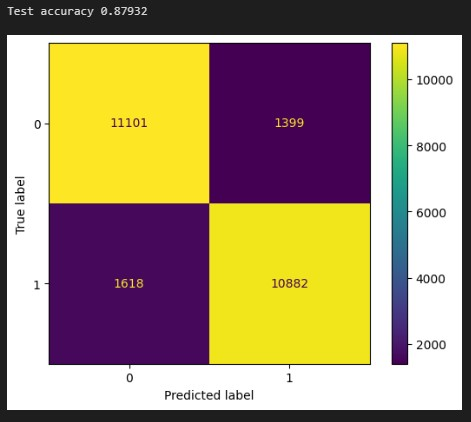
\includegraphics[scale=.70]{./test-GRU-[16]}
    \caption{\lr{GRU-[16]-[64, 16, 16]}}\label{fig.49}
\end{figure}





\begin{figure}[!h]
    \centering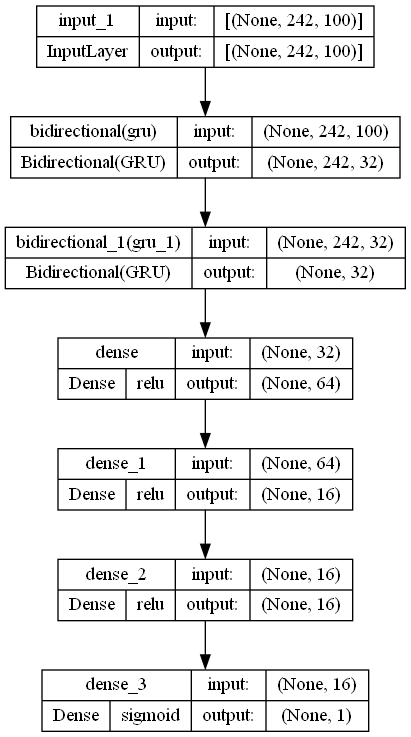
\includegraphics[scale=.45]{./GRU-[16, 16]}
    \caption{\lr{GRU-[16, 16]-[64, 16, 16]}}\label{fig.410}
\end{figure}


\begin{figure}[!h]
    \centering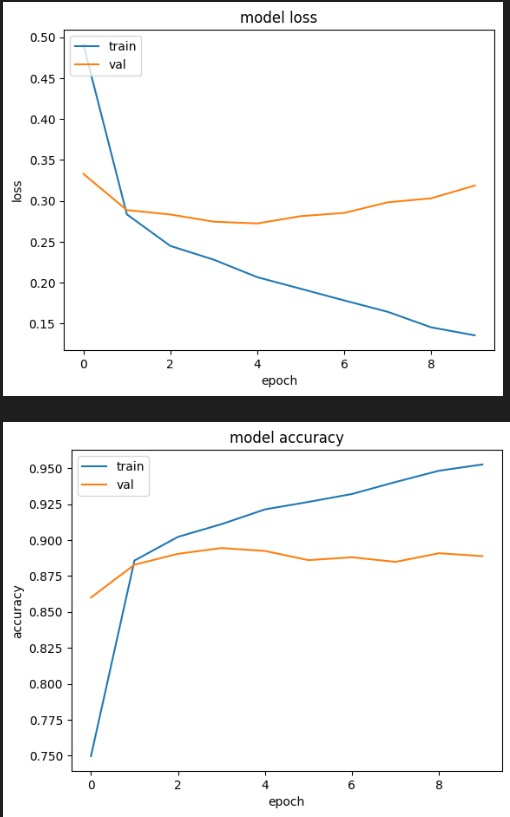
\includegraphics[scale=.65]{./GRU-[16, 16]-[64, 16, 16]}
    \caption{\lr{GRU-[16, 16]-[64, 16, 16]}}\label{fig.411}
\end{figure}


\begin{figure}[!h]
    \centering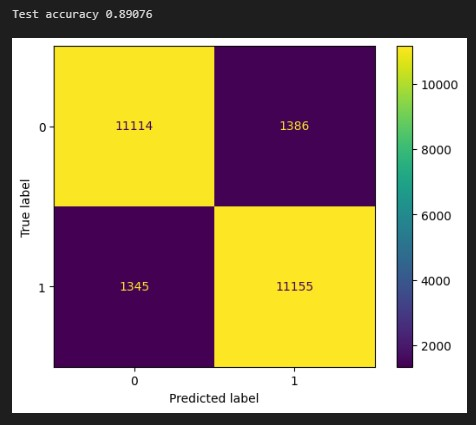
\includegraphics[scale=.70]{./test-GRU-[16, 16]}
    \caption{\lr{GRU-[16, 16]-[64, 16, 16]}}\label{fig.412}
\end{figure}




\cleardoublepage


همانطور که مشاهده می‌شود بهترین معماری مربوط به شبکه با دو لایه \lr{GRU} است که دقت داده‌های آزمون آن نزدیک به 90 درصد بدست آمد.

% -------------------------------------------------------------------

\section{سوال اضافی}
در این بخش با دو لایه کانولوشنی و 4 لایه پنهان شبکه به سرعت آموزش داده شد و دچار بیش‌برازش شد (99 درصد برای آموزش و نزدیک 80 درصد آزمون). به همین خاطر چندین لایه \lr{drop out} اضافه شد و نتایج زیر بدست آمد.

\begin{figure}[!h]
    \centering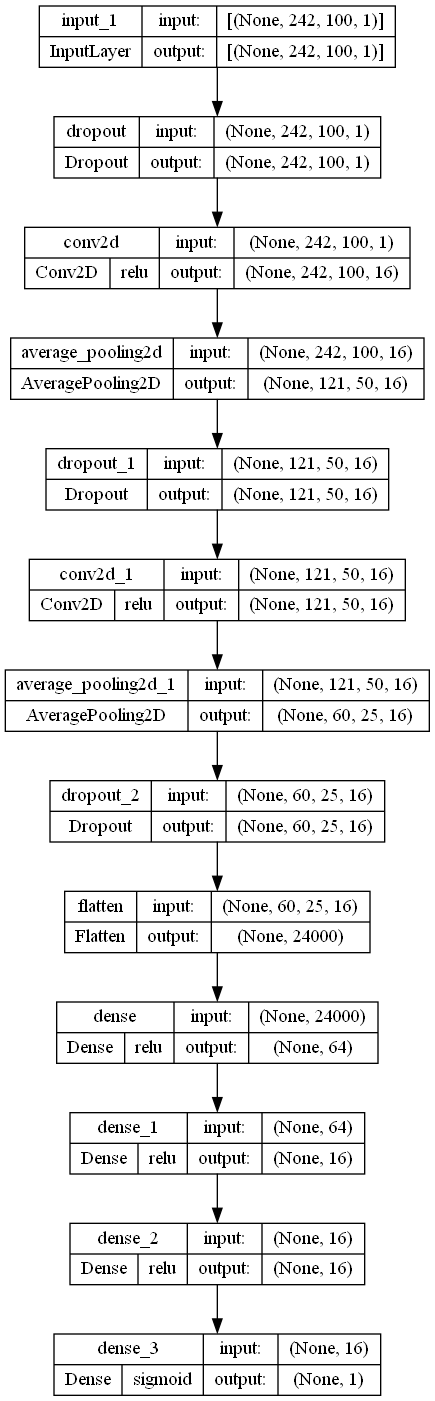
\includegraphics[scale=.45]{./cnn-}
    \caption{\lr{cnn}}\label{fig.51}
\end{figure}


\begin{figure}[!h]
    \centering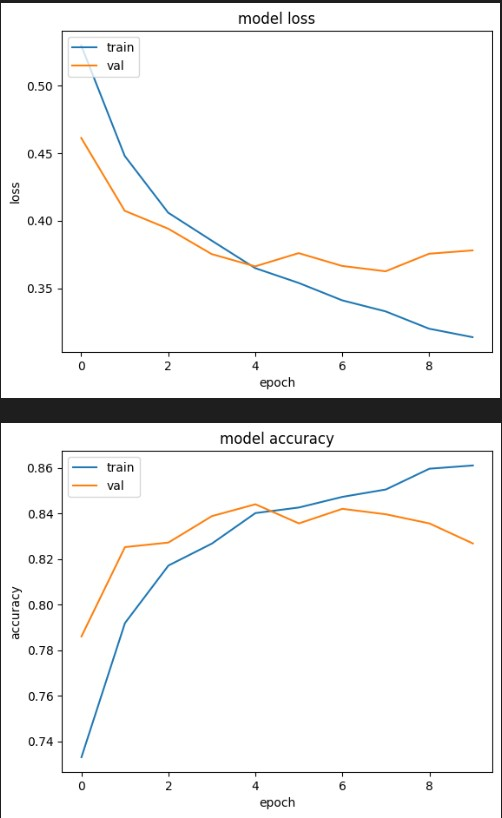
\includegraphics[scale=.65]{./cnn}
    \caption{\lr{cnn}}\label{fig.52}
\end{figure}


\begin{figure}[!h]
    \centering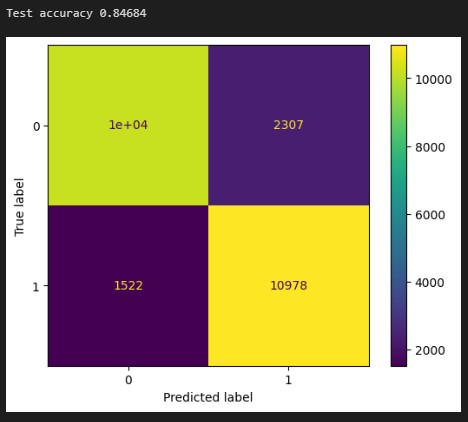
\includegraphics[scale=.70]{./test-cnn}
    \caption{\lr{cnn}}\label{fig.53}
\end{figure}



\cleardoublepage

همانطور که مشاهده می‌شود با تست یک شبکه کانولوشنی نتیجه نزدیکی به شبکه‌های بزگشتی گرفته شد. اما همچنان شبکه‌های بازگشتی با حداقل 5 درصد بهتر عمل کردند.


% -------------------------------------------------------------------

\end{document}